\documentclass[11pt]{article}

\usepackage[margin=1in]{geometry}
\usepackage{amsmath,amssymb,amsthm,mathrsfs}
\usepackage{graphicx}
\usepackage[hidelinks]{hyperref}

\newtheorem{theorem}{Theorem}

\newcommand{\ellp}{\ell_p}
\newcommand{\ellone}{\ell_1}
\newcommand{\cnull}{c_0}
\newcommand{\Fb}{\mathscr{F}_b}
\newcommand{\Fnull}{\mathscr{F}_0}

\begin{document}

\begin{center}
{\Large Literature status: unique asymptotic models need not yield
Asymptotic \(\ell_p\) subspaces}

\medskip
{\small Run \texttt{fa\_banach\_001}; source arXiv:math/0110146}
\end{center}

\section*{Source question}

Halbeisen and Odell's paper \emph{On asymptotic models in Banach spaces}
asks the following question in its open-problem section.

\begin{figure}[h]
\centering

\includegraphics[width=\textwidth]{figures/open_problem_crop.png}
\caption{arXiv:math/0110146, page 31, item (5.2.1).  The source TeX labels
the same item as Problem 6.1.}
\end{figure}

In words, suppose there are \(K\) and \(1\leq p\leq\infty\) such that every
asymptotic model of \(X\) is \(K\)-equivalent to the unit vector basis of
\(\ell_p\), with \(\cnull\) replacing \(\ell_\infty\).  Must \(X\) contain an
asymptotic \(\ell_p\) or \(\cnull\) subspace?

\section*{Supporting literature status}

Argyros, Georgiou, Manoussakis, and Motakis explicitly state that their paper
\emph{The complete separation of the two finer asymptotic \(\ell_p\)
structures for \(1\leq p<\infty\)} provides an answer to the corresponding
Halbeisen--Odell problem.

\begin{figure}[h]
\centering
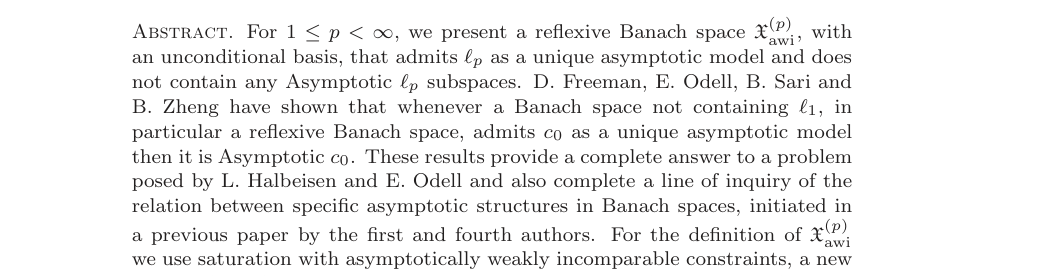
\includegraphics[width=\textwidth]{figures/supporting_abstract_complete_answer_crop.png}
\caption{arXiv:2106.12323, page 1: the abstract states the finite-\(p\)
construction and says that, together with the \(\cnull\) result of
Freeman--Odell--Sari--Zheng, it gives a complete answer to the
Halbeisen--Odell problem.}
\end{figure}

\begin{figure}[h]
\centering
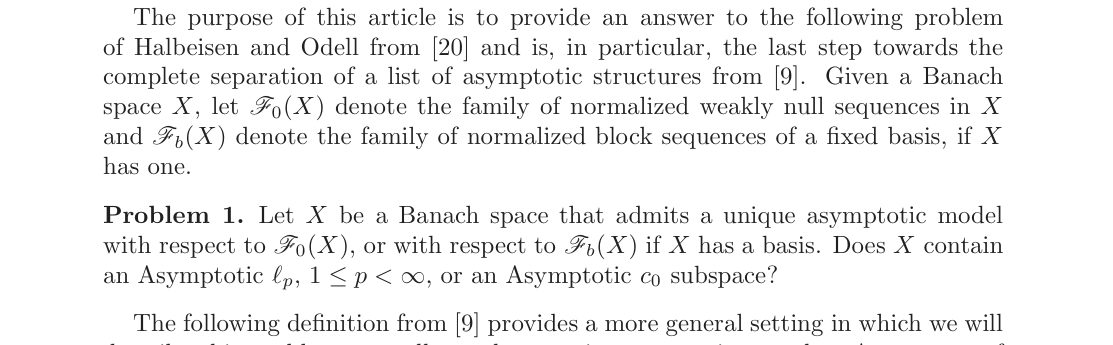
\includegraphics[width=\textwidth]{figures/supporting_problem_restatement_crop.png}
\caption{arXiv:2106.12323, page 2: the supporting paper restates the
Halbeisen--Odell problem for unique asymptotic models.}
\end{figure}

\begin{figure}[h]
\centering
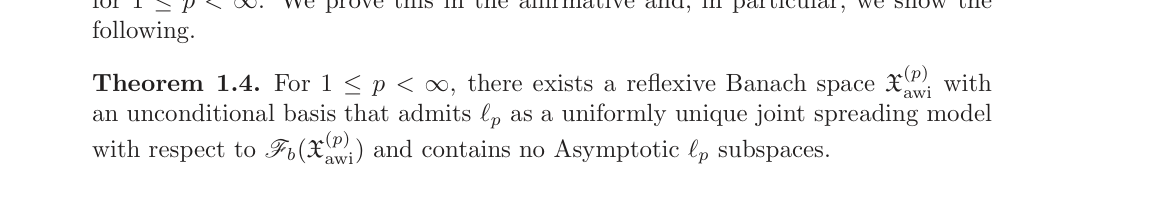
\includegraphics[width=\textwidth]{figures/supporting_theorem_1_4_crop.png}
\caption{arXiv:2106.12323, page 3: Theorem 1.4 gives the finite-\(p\)
counterexample.}
\end{figure}

\section*{Proof intuition}

The source problem asks whether array-level asymptotic uniqueness forces a
global asymptotic game structure in some subspace.  The later construction
separates these two notions.  The norm is saturated with asymptotically weakly
incomparable constraints so that arrays of normalized blocks still generate
only \(\ell_p\) as an asymptotic model, while each infinite-dimensional
subspace contains tree segments whose norm is too small to satisfy an
Asymptotic \(\ell_p\) lower estimate.  Thus the array property survives, but
the hereditary global asymptotic property fails.

\section*{The literature answer}

\begin{theorem}
For each \(1\leq p<\infty\), the finite-\(p\) part of Halbeisen--Odell's
Problem 6.1 has a negative answer.  There is a reflexive Banach space with an
unconditional basis that admits \(\ell_p\) as a unique asymptotic model with
respect to normalized block sequences, yet contains no Asymptotic \(\ell_p\)
subspace.
\end{theorem}

\begin{proof}
The supporting paper defines the hereditary properties
\((a)_p\) and \((b)_p\), where \((a)_p\) is being Asymptotic \(\ell_p\), and
\((b)_p\) is admitting \(\ell_p\) as a uniformly unique joint spreading model,
equivalently as a unique asymptotic model, with respect to \(\Fb(X)\)
\cite{AGMM}.  It then says that the only remaining open question in the
separation diagram is whether \((b)_p\) completely separates from \((a)_p\)
for \(1\leq p<\infty\), and proves this affirmatively.

Concretely, Theorem 1.4 of \cite{AGMM} states that for every
\(1\leq p<\infty\) there exists a reflexive Banach space
\(\mathfrak X_{\mathrm{awi}}^{(p)}\) with an unconditional basis that admits
\(\ell_p\) as a uniformly unique joint spreading model with respect to
\(\Fb(\mathfrak X_{\mathrm{awi}}^{(p)})\) and contains no Asymptotic
\(\ell_p\) subspaces.  By the equivalence between uniformly unique joint
spreading models and unique asymptotic models recalled in the same paper,
\(\mathfrak X_{\mathrm{awi}}^{(p)}\) satisfies the asymptotic-model
hypothesis of the Halbeisen--Odell question in the finite-\(p\), block-array
setting.  The conclusion asked for in the problem fails because the space has
no Asymptotic \(\ell_p\) subspace at all.

The abstract of \cite{AGMM} also records the complementary \(\cnull\) side:
Freeman, Odell, Sari, and Zheng proved that whenever a Banach space not
containing \(\ellone\), in particular a reflexive Banach space, admits
\(\cnull\) as a unique asymptotic model, it is Asymptotic \(\cnull\).
Thus the finite-\(p\) answer is negative, while the \(\cnull\) answer is
positive under the standard no-\(\ellone\) hypothesis.
\end{proof}

\section*{Verification notes and limitations}

This packet is a literature-status identification, not a new proof.  The
supporting paper explicitly names Halbeisen and Odell, restates their problem,
and says its results provide a complete answer.

The source paper's item (5.2.1) is phrased for asymptotic models being
\(K\)-equivalent to \(\ell_p\) or \(\cnull\).  The supporting theorem gives the
stronger uniqueness/equivalence-to-\(\ell_p\) hypothesis for normalized block
arrays and a reflexive counterexample to the requested Asymptotic \(\ell_p\)
subspace conclusion.  This settles the finite-\(p\) direction in the standard
block-array interpretation used by the later paper.

The run lightweight indexes were searched for arXiv:0110146 and the key
phrases ``asymptotic model'', ``Halbeisen'', ``Odell'', ``normalized weakly
null'', and ``spreading model''.  No existing exact packet for this problem was
found.  A local primary-source search then found arXiv:2106.12323 via the
phrases ``Halbeisen and Odell'', ``complete answer'', and ``unique asymptotic
model''.

\section*{Human review recommendation}

Treat the finite-\(p\) part of Halbeisen--Odell Problem 6.1 as already
answered negatively by \cite{AGMM}.  Keep this packet as duplicate/status
memory and do not count it as an original proof from this run.  Other open
problems in the Halbeisen--Odell section remain outside this packet.

\begin{thebibliography}{9}

\bibitem{HO}
L. Halbeisen and E. Odell,
\emph{On asymptotic models in Banach spaces},
Israel J. Math. 139 (2004), 253--291; arXiv:math/0110146.

\bibitem{AGMM}
S. A. Argyros, A. Georgiou, A. Manoussakis, and P. Motakis,
\emph{The complete separation of the two finer asymptotic \(\ell_p\)
structures for \(1\leq p<\infty\)},
arXiv:2106.12323.

\bibitem{FOSZ}
D. Freeman, E. Odell, B. Sari, and B. Zheng,
\emph{On spreading sequences and asymptotic structures},
Trans. Amer. Math. Soc. 370 (2018), no. 10, 6933--6953.

\end{thebibliography}

\end{document}
